\chapter{Distributed computing}
As mentioned, low scalability is a problem in a Siemens windmill farm. The Wind Power Supervisor (WPS) and the Park Regulator does not scale well with the number of turbines, which introduces performance issues to the solution. Both in terms handling external requests, which is done by the WPS, but also when regulating the windmill farm through the Park Regulator. 

An example of this is the Regulator calculation sequence illustrated on \cref{fig:dataComputationSequence}. Today this sequence takes approximately 150 ms. Siemens wishes this time reduced to 10 ms.

When distributing the Wind Power Supervisor onto the turbines, the turbines obviously needs to be able to handle these external requests and windmill farm regulations. For the heavy tasks, in terms of CPU power, distributed computing becomes relevant as a way of improving performance by combining the CPU power residing inside the turbines to compute a common task. 

In distributed computing, each node or process has its own local memory and communication happens via message passing \cite{andrews2000foundations}. This chapter describes relevant distributed computing communication paradigms and discusses which technology that is the best for the Siemens case. 


\section{Message passing}

Message passing is a low-level communication paradigm, where processors communicate by sending messages via bidirectional channels. It's a highly used paradigm and other communication paradigms are usually implemented on top of an underlying message-passing system.  

With message passing being a low-level communication paradigm, the communication overhead is low compared to paradigms build on top of it. It is entirely up to the application developer to handle communication. This will in many cases result in better performance, which is the most compelling argument for choosing message passing as communication paradigm. The problem with it being up to the developer, is that the developer needs to deal with configurations setup, exception handling, who and when to communicate with, etc., when developing the application. This makes it hard to develop using message passing, compared to distributed shared memory, especially when dealing with more complex applications \cite{lu1995message}. 

%Results?


%\section{Shared memory}
%
%In a shared memory system, several nodes communicate via a global memory area that contains a set of shared variables. This paradigm (illustrated on \cref{fig:sharedMemorySystem}) is an extension of message passing and requires a server or node dedicated to the global memory area.
%
%\begin{figure}
%	\centering
%	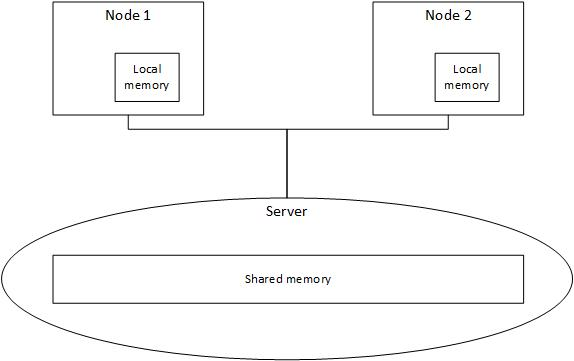
\includegraphics[width=0.8\textwidth,natwidth=610,natheight=642]{SharedMemory.jpg} 
%	\captionsetup{format=plain,font=footnotesize,labelfont={bf,defaultCapFont},labelsep=quad,singlelinecheck=no}
%	\caption[Distributed Computing System with 2 nodes]{
%		\label{fig:sharedMemorySystem} 
%		\footnotesize{%
%			A shared memory system with 2 nodes.
%		}
%	}
%\end{figure}



\section{Distributed shared memory}

Shared memory is an attractive paradigm for designing parallel and distributed systems. Applications can use shared memory as a tool for the entire system to share a common state. However for loose coupled distributed systems, no physically shared memory is available to support such a model. Distributed shared memory (DSM) is a way of providing physically distributed memory machines a shared memory abstraction, illustrated on \cref{fig:distributedSharedMemory}.

\begin{figure}
	\centering
	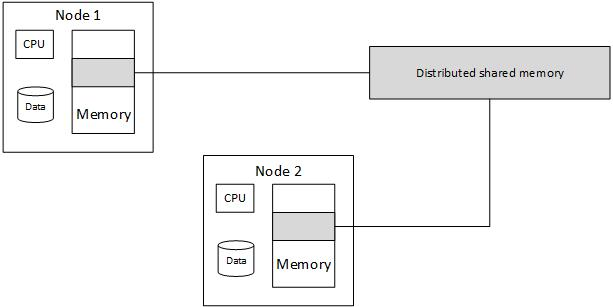
\includegraphics[width=0.8\textwidth,natwidth=610,natheight=642]{DistributedSharedMemory.jpg} 
	\captionsetup{format=plain,font=footnotesize,labelfont={bf,defaultCapFont},labelsep=quad,singlelinecheck=no}
	\caption[Distributed Computing System with 2 nodes]{
		\label{fig:distributedSharedMemory} 
		\footnotesize{%
			A distributed shared memory system with 2 nodes.
		}
	}
\end{figure}

The primary advantage of DSM over message passing is the shared memory abstraction provided. This gives the illusion of physically shared memory and allows developers to use the shared-memory paradigm, without having to think about communication mechanisms. However the abstraction also introduces overhead to the system, which decreases performance. The DSM abstraction has limited knowledge of the application flow of the application, compared to communication via message passing. 
 
Comparing DSM with message passing with regards to performance is not entirely fair since DSM is build on top of message passing. However the comparison is necessary when considering what technology to use for a given system and in this case, the comparison results in a trade off between performance and the shared memory abstraction. 

Honghui \cite{lu1995message} has studied the trade-off between message passing performance and the shared memory abstraction. He ported nine different parallel programs to a DSM system called ThreadMarks and a message passing system called PVM and compared the two technologies with regards to programmability and performance. He argues that given DSM is an abstraction built on top of message passing, DSM cannot achieve better performance than message passing. Therefore the goal is to achieve the same performance as message passing using DSM. 




\section{Publish/subscribe}


\section{Remote message invocation}


\section{Conclusion}

%Ens
%Valg med vægt på arkitektur og development tid. 
%RMI fravalg